\documentclass[t]{beamer}
% \documentclass[handout,xcolor=pdftex,dvipsnames,table]{beamer}

\mode<presentation>
{
  \usetheme{Warsaw}
  \usecolortheme{whale}
  % or ...

  % or whatever (possibly just delete it)
  \setbeamertemplate{navigation symbols}{}
}

\usepackage{hyperref}

% make a command to decrease font size locally when desired
\newcommand\Fontvi{\fontsize{8.5}{7.2}\selectfont}



\setbeamertemplate{itemize items}[ball]
\setbeamertemplate{itemize subitem}[triangle]
\setbeamertemplate{itemize subsubitem}[circle]
\setbeamercovered{invisible}

\usepackage{palatino} 
\usepackage{listings} % Gives syntax highlighting for python code. 
\usepackage{color} % Used for syntax highlighting. 
\usepackage{textcomp} % Used for syntax highlighting. 
\usepackage{caption}
\captionsetup{labelformat=empty,labelsep=none}
% This gives syntax highlighting in the python environment 
\definecolor{gray}{gray}{0.5} 
\definecolor{key}{rgb}{0,0.5,0} 
\lstset{
language=python,
basicstyle=\ttfamily\tiny, 
otherkeywords={1, 2, 3, 4, 5, 6, 7, 8 ,9 , 0, -, =, +, [, ], (, ), \{, \}, :, *, !}, 
keywordstyle=\color{blue}, 
stringstyle=\color{red},
showstringspaces=false,
alsoletter={1234567890},
otherkeywords={\ , \}, \{},
keywordstyle=\color{blue},
emph={access,and,break,class,continue,def,del,elif ,else,%
except,exec,finally,for,from,global,if,import,in,is,%
lambda,not,or,pass,print,raise,return,try,while},
emphstyle=\color{black}\bfseries,
emph={[2]True, False, None, self},
emphstyle=[2]\color{green},
emph={[3]from, import, as},
emphstyle=[3]\color{blue},
upquote=true,
morecomment=[s]{"""}{"""},
commentstyle=\color{gray}\slshape,
emph={[4]1, 2, 3, 4, 5, 6, 7, 8, 9, 0},
emphstyle=[4]\color{blue},
literate=*{:}{{\textcolor{blue}:}}{1}%
{=}{{\textcolor{blue}=}}{1}%
{-}{{\textcolor{blue}-}}{1}%
{+}{{\textcolor{blue}+}}{1}%
{*}{{\textcolor{blue}*}}{1}%
{!}{{\textcolor{blue}!}}{1}%
{(}{{\textcolor{blue}(}}{1}%
{)}{{\textcolor{blue})}}{1}%
{[}{{\textcolor{blue}[}}{1}%
{]}{{\textcolor{blue}]}}{1}%
{<}{{\textcolor{blue}<}}{1}%
{>}{{\textcolor{blue}>}}{1},%
numbers=none,
}

\newcommand{\putat}[3]{\begin{picture}(0,0)(0,0)\put(#1,#2){#3}\end{picture}}



\title[]{Python Workshop\\
Process Flow}

\author[Hughes] % (optional, use only with lots of authors)
{Joseph D.~Hughes}
\institute[USGS] % (optional, but mostly needed)
{
  U.S. Geological Survey\\
  Florida Water Science Center, Tampa, Florida USA
  }
  \titlegraphic{
\includegraphics[scale=0.5]{figures/c_USGSid1.pdf}}
  

\date[UQ12] % (optional, should be abbreviation of conference name)
{USGS National Groundwater Workshop, August 2012}

\subject{Python}


\begin{document}

\begin{frame}
  \titlepage
\end{frame}
\logo{\vspace{-0.3cm} 
\includegraphics[width=1.5cm]{figures/c_USGSid1.pdf}\hspace*{11.10cm}}  

\begin{frame}{Outline}
\tableofcontents
\end{frame}

\begin{frame}[fragile]
\frametitle{Overview}
\begin{itemize}

\item Much of what is useful to do in Python is reading files, manipulating the data, and writing out results in another format
\item Python and Numpy provide ways to read and write ASCII and binary files. We will focus on ASCII files
\end{itemize}
\end{frame}

\begin{frame}[fragile]
\frametitle{Background Information}
Process flow control resources: \\
\href{http://docs.python.org/tutorial/controlflow.html}{\texttt{\small{\textcolor{blue}{http://docs.python.org/tutorial/controlflow.html}}}}
\end{frame}

\begin{frame}{\texttt{\textbf{while}}, \texttt{\textbf{continue}}, and \texttt{\textbf{break}}}
\texttt{ProcessFlowExamples.py} \\ Import data from an external file and iterate over data using \texttt{\textbf{while}} and \texttt{\textbf{print}} last entry.
  \begin{figure}[ht]
  \centering
        \lstset{numbers=left}
        \lstinputlisting[language=python, firstline=1,lastline=18]{python/ProcessFlowExamples.py}
   \end{figure}
\end{frame}

\begin{frame}{\texttt{\textbf{range}} iterator and \texttt{\textbf{continue}}}
\texttt{ProcessFlowExamples.py} \\ Import data from an external file and iterate over data using \texttt{\textbf{range}}  and \texttt{\textbf{print}}  last entry.
  \begin{figure}[ht]
  \centering
        \lstset{numbers=left}
        \lstinputlisting[language=python, firstline=1,lastline=5]{python/ProcessFlowExamples.py}
       $\vdots$
        \lstinputlisting[language=python, firstline=19,lastline=25,firstnumber=19]{python/ProcessFlowExamples.py}
   \end{figure}
\end{frame}

\begin{frame}{\texttt{\textbf{xrange}} iterator and \texttt{\textbf{continue}}}
\texttt{ProcessFlowExamples.py} \\ Import data from an external file and iterate over data using \texttt{\textbf{xrange}}  and \texttt{\textbf{print}}  last entry.
  \begin{figure}[ht]
  \centering
        \lstset{numbers=left}
        \lstinputlisting[language=python, firstline=1,lastline=5]{python/ProcessFlowExamples.py}
       $\vdots$
        \lstinputlisting[language=python, firstline=26,lastline=32,firstnumber=26]{python/ProcessFlowExamples.py}
   \end{figure}
\end{frame}

\begin{frame}{\texttt{\textbf{in}} iterator and \texttt{\textbf{continue}}}
\texttt{ProcessFlowExamples.py} \\ Import data from an external file and iterate over data using \texttt{\textbf{in}} iterator and \texttt{\textbf{print}}  last entry.
  \begin{figure}[ht]
  \centering
        \lstset{numbers=left}
        \lstinputlisting[language=python, firstline=1,lastline=5]{python/ProcessFlowExamples.py}
       $\vdots$
        \lstinputlisting[language=python, firstline=33,lastline=42,firstnumber=33]{python/ProcessFlowExamples.py}
   \end{figure}
\end{frame}

\begin{frame}{\texttt{\textcolor{red}{enumerate}} iterator and \texttt{\textbf{continue}}}
\texttt{ProcessFlowExamples.py} \\ Import data from an external file and iterate over data using \texttt{\textcolor{red}{enumerate}} iterator and \texttt{\textbf{print}}  last entry.
  \begin{figure}[ht]
  \centering
        \lstset{numbers=left}
        \lstinputlisting[language=python, firstline=1,lastline=5]{python/ProcessFlowExamples.py}
       $\vdots$
        \lstinputlisting[language=python, firstline=43,lastline=49,firstnumber=43]{python/ProcessFlowExamples.py}
   \end{figure}
\end{frame}

\begin{frame}[fragile]
\frametitle{\texttt{ProcessFlowExamples.py} output}
  \begin{figure}[ht]
  \centering
        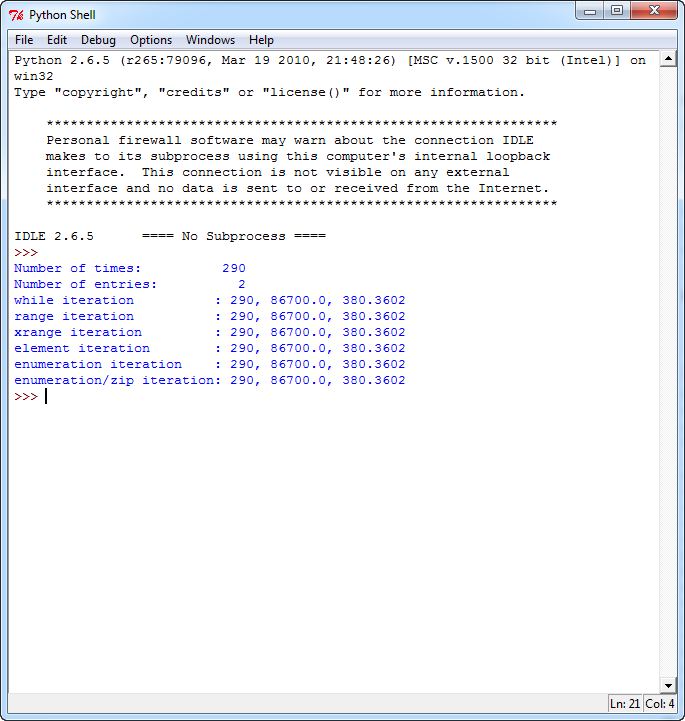
\includegraphics[height=0.85\textheight]{figures/ProcessFlowExamplesPythonShellOutput}
   \end{figure}
\end{frame}

\end{document}